\documentclass{beamer}
\usetheme{MasterII}

\usepackage{macros}

\title{Optimizing application performance \\ through optimizing compilation}
\author{Francois Flandin}
\supervisor{Pr Sid Touati}
\date{First semester of year 2024-2025}

\newcommand{\gcc}{\texttt{gcc} }
\newcommand{\icx}{\texttt{icx} }
\newcommand{\clang}{\texttt{clang} }
\newcommand{\comp}{\texttt{ccomp} }
\newcommand{\optizero}{\texttt{-O0} }
\newcommand{\optione}{\texttt{-O1} }
\newcommand{\optitwo}{\texttt{-O2} }
\newcommand{\optithree}{\texttt{-O3} }
\newcommand{\optisize}{\texttt{-Os} }
\newcommand{\clgg}{\texttt{C}}
\newcommand{\cpp}{\texttt{C++}}

\begin{document}
    
    \maketitle
    
    \section{Introduction}
    \begin{frame}{Introduction}
        \begin{block}{Objective}
            Explore how compilers optimizes programs using several optimizations levels : \optizero, \optione, \optitwo, \optithree, \optisize.
        \end{block}
        \begin{block}{2 parts to the project}
            \begin{enumerate}
            \item Compiling 2 programs in \clgg/\cpp with each optimization level and compiler to compare performances
            \item Checking which optimization is enabled for each optimization level and compiler
            \end{enumerate}
        \end{block}
    \end{frame}
    
    \begin{frame}[noframenumbering]{Content}
        \tableofcontents
    \end{frame}
    
    \section{Experience}
    \begin{frame}[noframenumbering]{Content}
        \tableofcontents[currentsection]
    \end{frame}
    
    \subsection{Environnement}
    \begin{frame}{Architecture}
        \begin{block}{}
            \begin{description}
                \item[Model name: ] 11th Gen Intel Core i5-1135G7 @ 2.40GHz
                \item[Adress size: ] 39 bits physical, 48 bits virtual
                \item[Cache line size: ] 64 bytes
                \item[Physical cores: ] 4
            \end{description}
        \end{block}
        
        \begin{block}{}
            \begin{table}[H]
                \centering
                \begin{tabular}{|l|c|c|c|c|}
                    \hline
                    Cores & 0  4 & 1  5 & 2  6 & 3  7 \\
                    \hline
                    L1 Cache & 48 kB & 48 kB & 48 kB & 48 kB \\
                    \hline
                    L2 Cache & 1MB & 1MB & 1MB & 1MB \\
                    \hline
                    L3 Cache & \multicolumn{4}{|c|}{8 MB} \\
                    \hline
                \end{tabular}
                \caption{Computer's topology}
                \label{tab:graph_characteristics}
            \end{table}
        \end{block}
    \end{frame}
    
    
    \begin{frame}{Software}
        \begin{block}{Configuration}
            Computer in a lighweight configuration, avoid OS's optimizations and bloat from other programs or graphical interface.
        \end{block}
        \begin{block}{OS and compilers}
            \begin{description}
                \item[OS: ] Fedora Linux Workstation v40
                \item[gcc: ] version 14.2.1
                \item[icx: ] version 2024.2.1
                \item[clang: ] version 18.1.8
                \item[ccomp: ] version 3.14
            \end{description}
        \end{block}
    \end{frame}
    
    \subsection{Method}
    
    \begin{frame}{Experience Method}
        \begin{block}{Programs}
            There are 2 programs to compile : Matrix Multiplication (\clgg) and Dijkstra's algorithm (\cpp). For each compiler and optimization level.
        \end{block}
        \begin{block}{Object Size}
            The matrix size is set to two times the size of the largest cache. \newline
            The graph size is really huge to have a significate execution time.
        \end{block}
        \begin{block}{Mesurement}
            Function \texttt{gettimeofday()} placed before and after the main computation, mesuring initialisation time is not the goal.
        \end{block}
        \begin{block}{Finally}
            Run each program 12 times to visualize the data with R
        \end{block}
            
    \end{frame}
    
    \section{Results}
    \begin{frame}[noframenumbering]{Content}
        \tableofcontents[currentsection]
    \end{frame}
    
    \subsection{Matrix Multiplication}
    \begin{frame}{Matrix Multiplication Results}
        \begin{figure}[H]
        \centering
        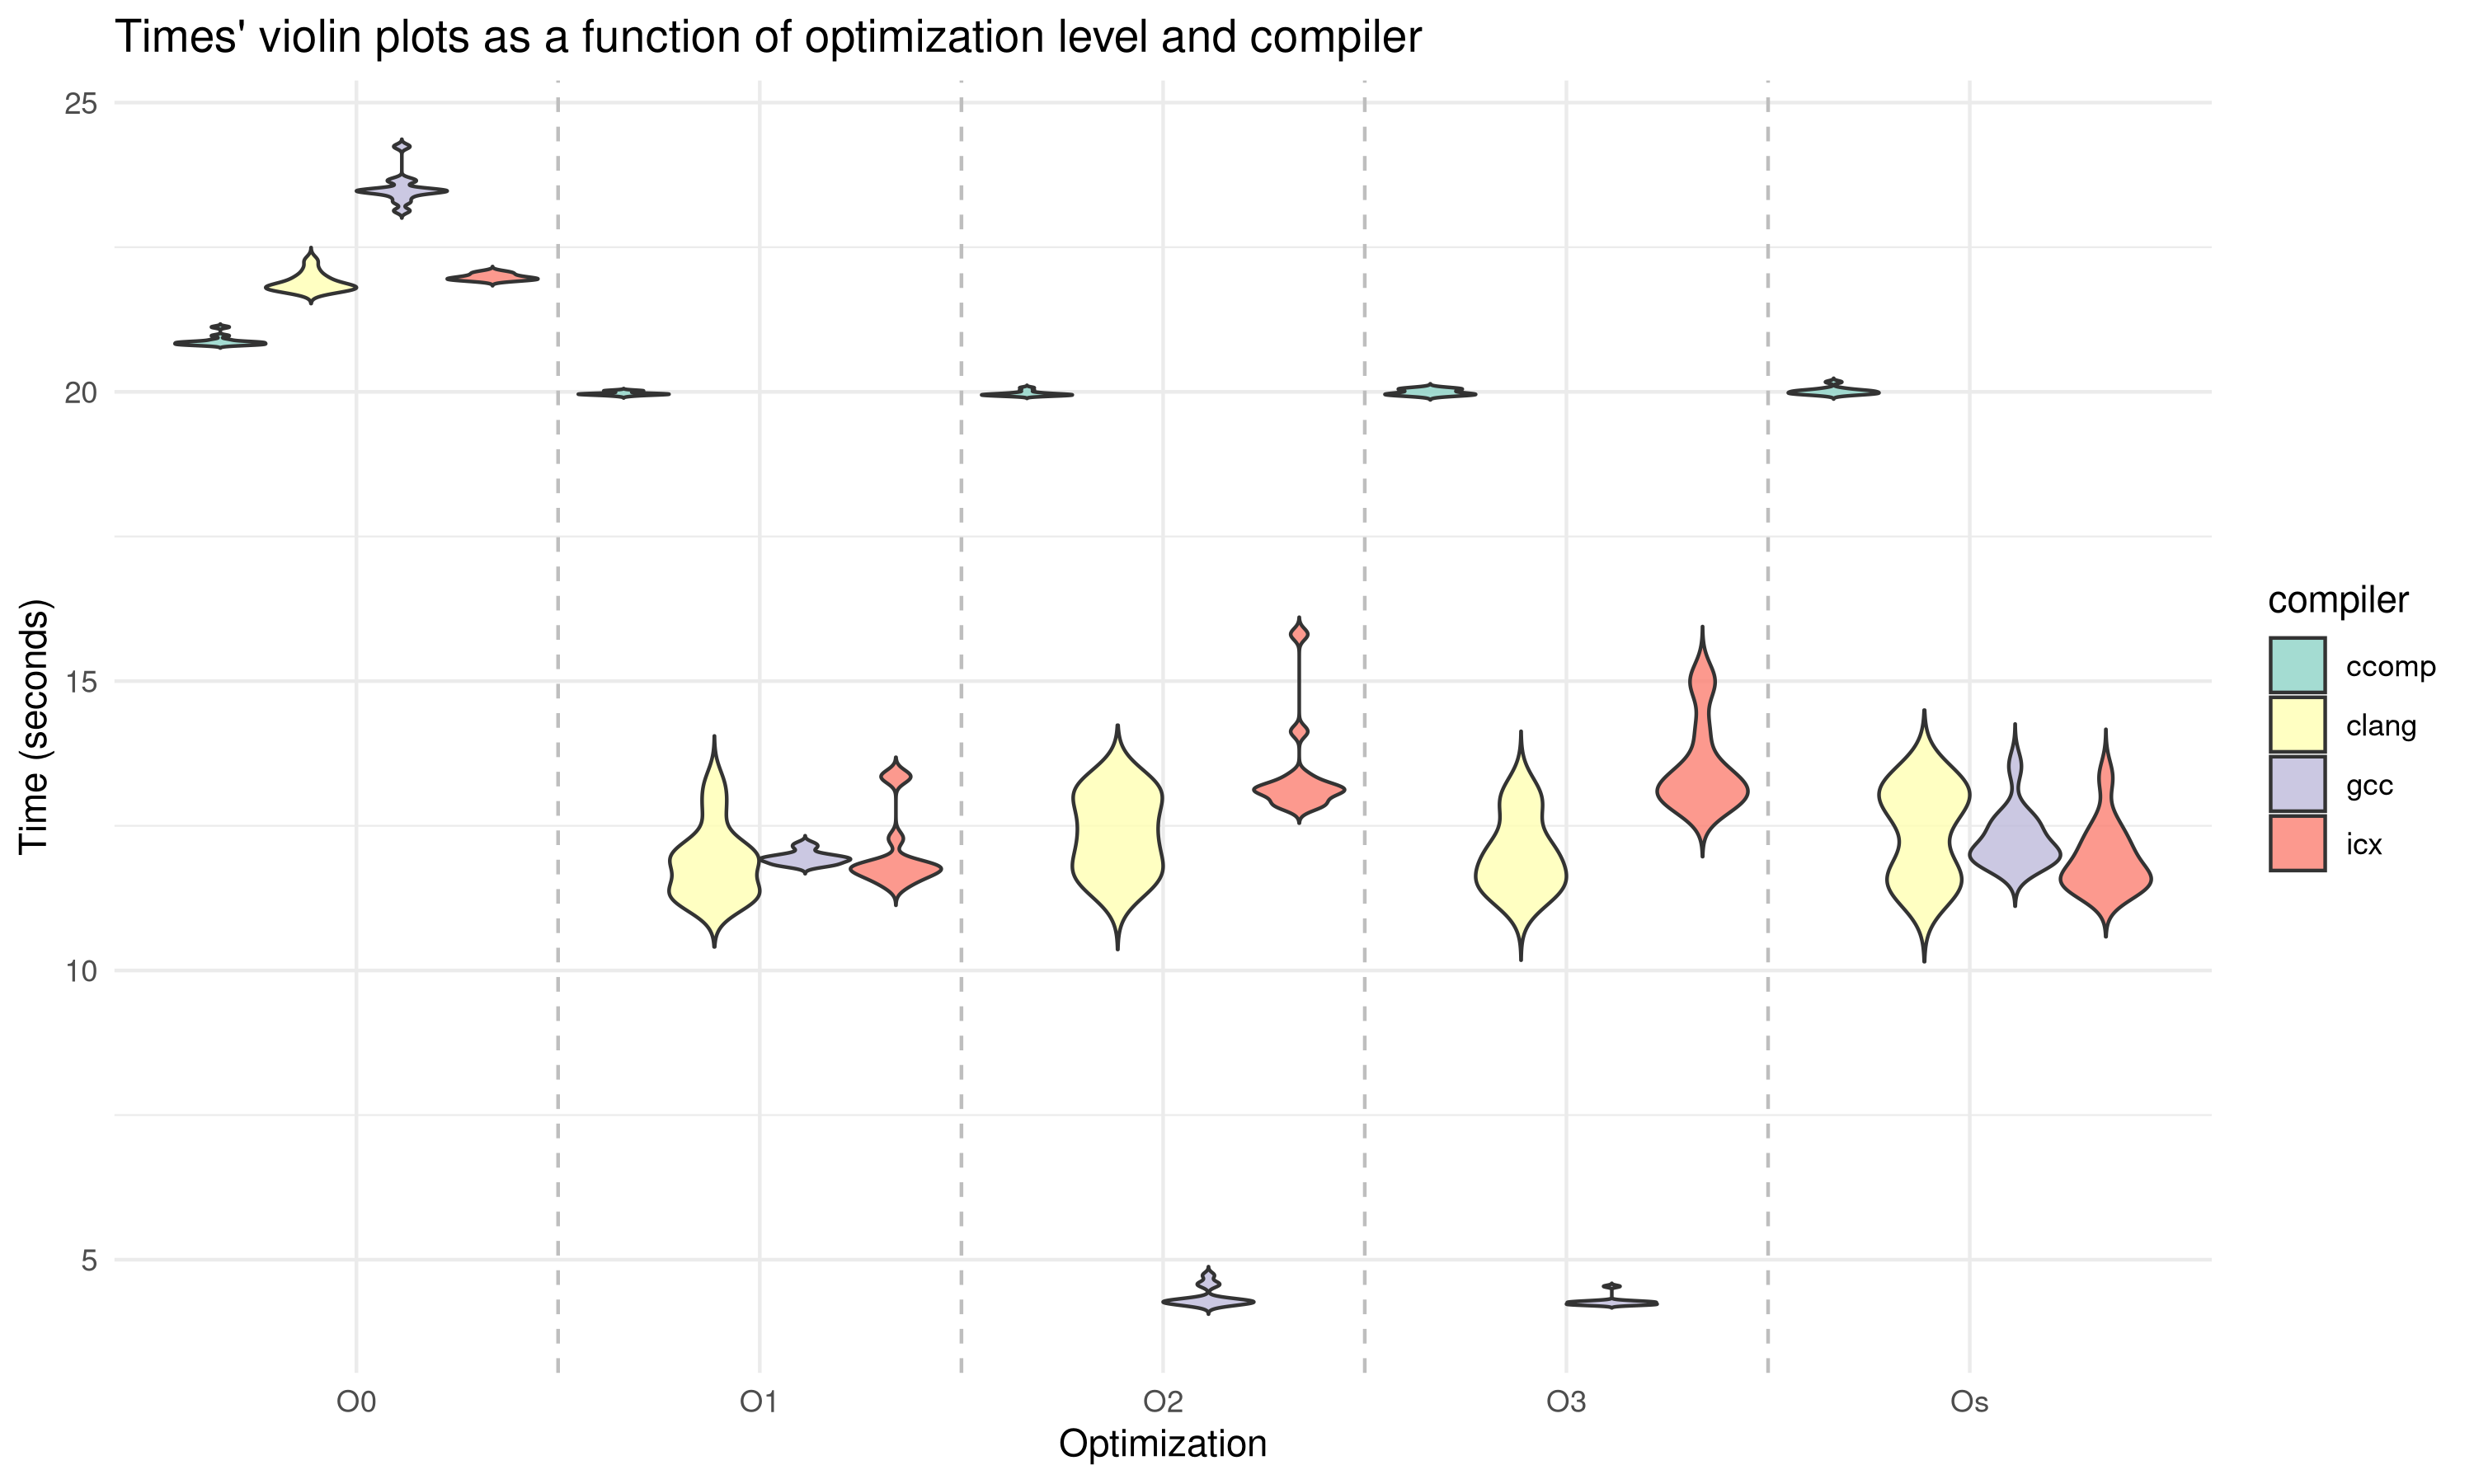
\includegraphics[width=1\textwidth]{img/plots/violin_plot_mat_mult.png}
        \caption{Evolution of the execution time of the program mat\_mult.c as a function of compiler and optimization level.}
        \label{fig:image1}
        \end{figure}
    \end{frame}
    
    \subsection{Dijkstra}
    \begin{frame}{Dijkstra Results}
        \begin{figure}[H]
        \centering
        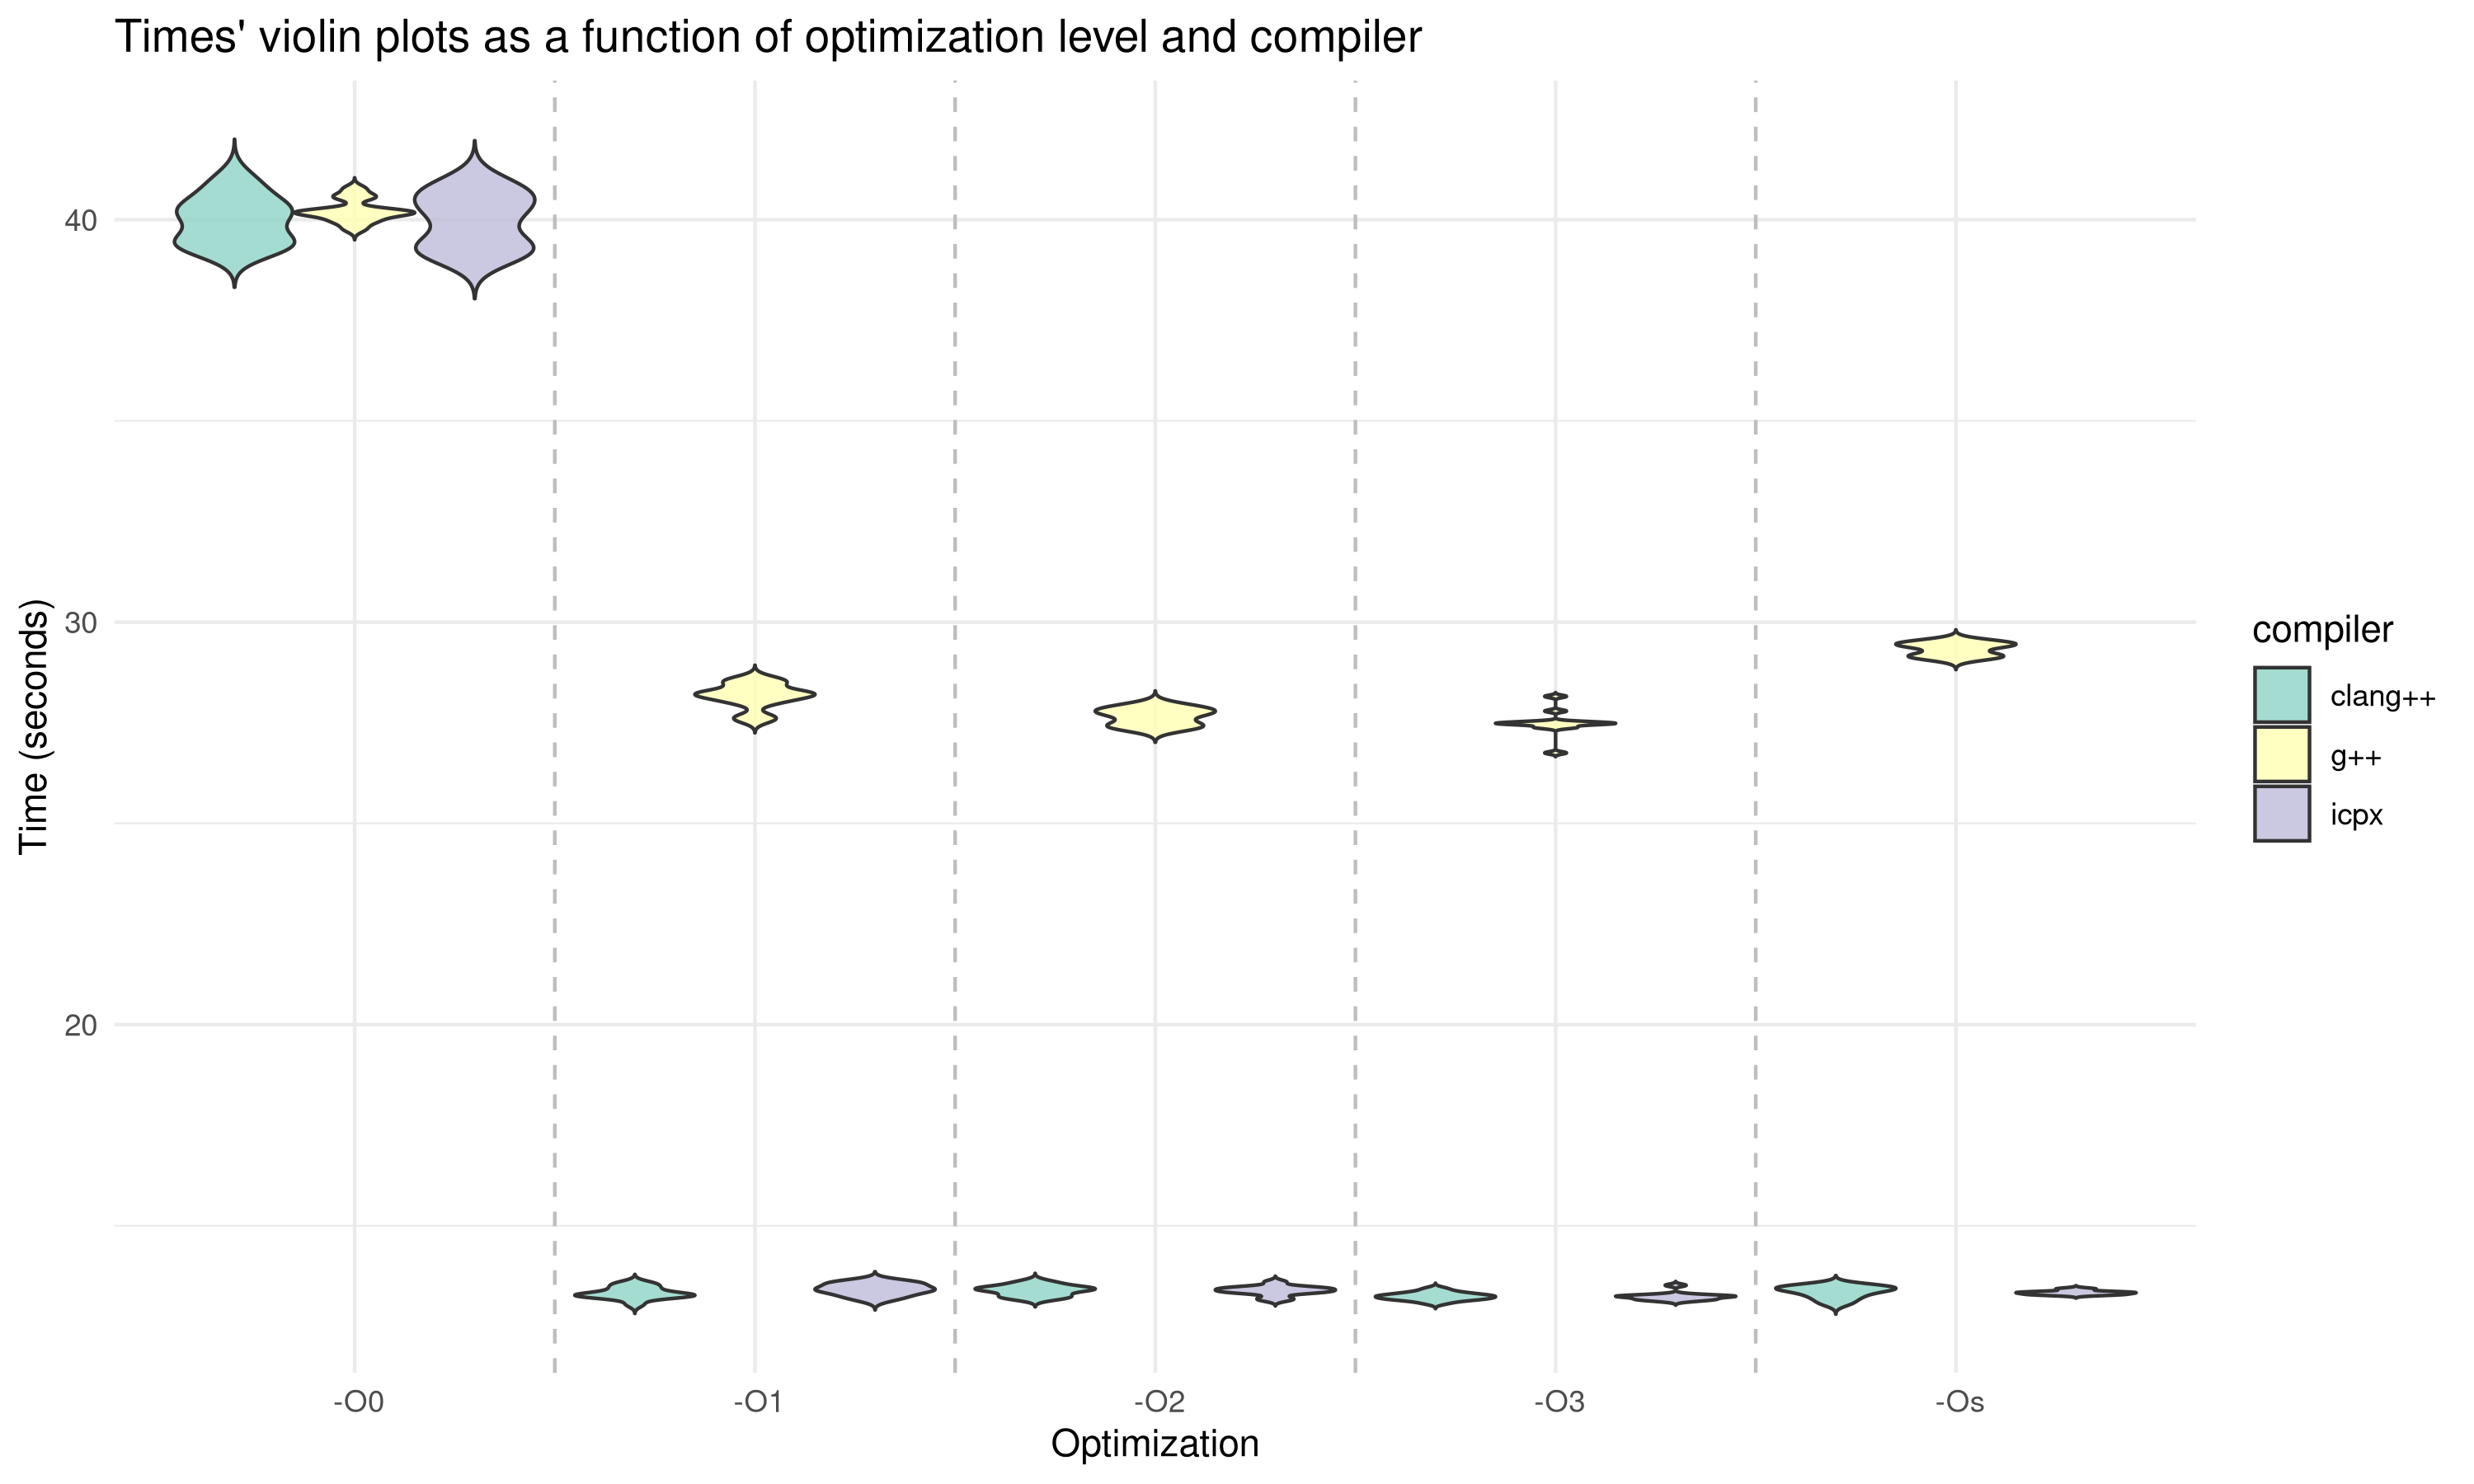
\includegraphics[width=1\textwidth]{img/plots/violin_plot_dijkstra.png}
        \caption{Evolution of the execution time of the program mat\_mult.c as a function of compiler and optimization level.}
        \label{fig:image2}
        \end{figure}
    \end{frame}
    
    \begin{frame}{Benchmarks Analysis}
        \begin{block}{}
            \begin{table}[H]
            \centering
            \begin{tabular}{|l|c|c|c|}
            \hline
            & \gcc & \clang & \icx \\
            \hline
            total time taken & 136.37s       & 146.98s       & 155.65s \\
            dijkstra usage   & $\approx19\%$ & $\approx9\%$  & $\approx11\%$    \\
            init/free usage  & $\approx81\%$ & $\approx91\%$ & $\approx89\%$   \\
            \hline
            \end{tabular}
            \end{table}
        \end{block}
    \end{frame}
    
    \section{Compilers Optimization}
    \begin{frame}[noframenumbering]{Content}
        \tableofcontents[currentsection]
    \end{frame}
    
    \subsection{How to get Compilers' Optimizations ?}
    \begin{frame}[fragile]{How to get Compilers' Optimizations ?}
        \begin{block}{gcc}
            \texttt{gcc --help=optimizers -Q -On}
        \end{block}
        \begin{block}{clang}
            \texttt{clang -O2 -emit-llvm -S program.c -o program.ll} \newline
            \texttt{opt -O2 -debug-pass-manager program.ll -o program.ll}
        \end{block}
        \begin{block}{icx and ccomp}
            Everything is inside their documentation.
        \end{block}
    \end{frame}
    
    \subsection{Some compilation optimizations}
    
    \begin{frame}[<+->]{Global Optimizations}
        \begin{block}{Peephole optimizations}
            Optimize a program over a reduced windows that slides through the program.
        \end{block}
        \begin{block}{Strength reduction}
            Replace heavy computations with lighter ones.
        \end{block}
        \begin{block}{Code motion}
            Allow the compiler to move instructions around the program.
        \end{block}
        \begin{block}{Elimination of common subexpressions}
            Reuse previously computed values.
        \end{block}
    \end{frame}
    
    \begin{frame}[<+->]{Loop Optimizations}
        \begin{block}{Loop unrolling}
            Reduces loop overhead by duplicating loop's body several times.
        \end{block}
        \begin{block}{Loop interchange}
            Improve memory access by modifying the loops order in a serie of nested loops.
        \end{block}
        \begin{block}{Loop peeling}
            Simplifies loops by removing non changing computation out of the loop.
        \end{block}
        \begin{block}{Loop jamming/fusion}
            Combine two adjacent loops into a single loop.
        \end{block}
    \end{frame}
    
    \begin{frame}[<+->]{Code elimination}
        \begin{block}{Dead code elimination}
            Removes part of the code that are not used.
        \end{block}
        \begin{block}{Dead store elimination}
            Removes variable affectations that aren't used through the program.
        \end{block}
        \begin{block}{Dead static function elimination}
            Removes static functions that are never used.
        \end{block}
        \begin{block}{Dead argument elimination}
            Removes unused function arguments.
        \end{block}
    \end{frame}
    
    \begin{frame}[<+->]{Clang's coroutine's management}
        Coroutines in C++ are functions that can be paused and resumed, enabling asynchronous and cooperative task management.
        \begin{block}{CoroEarlyPass}
            Prepares coroutine constructs by splitting their code into manageable parts.
        \end{block}
        \begin{block}{CoroElidePass}
            Eliminates unnecessary coroutine frames when they are not required.
        \end{block}
        \begin{block}{CoroCleanupPass}
            Finalizes coroutine transformations by removing temporary constructs and generating efficient, optimized code.
        \end{block}

    \end{frame}
    
    \begin{frame}[<+->]{What about ccomp ?}
        Does not activate much, but it has its optimizations !
        \begin{block}{Constant propagation}
            Replace constant variable calls with the value.
        \end{block}
        \begin{block}{Common subexpression elimination}
            Reuse previously computed values.
        \end{block}
        \begin{block}{Inlining}
            Replace function calls with function's body.
        \end{block}
    \end{frame}
    
    \begin{frame}{Conclusion: Each compiler has its pros}
        \begin{block}{\gcc}
            We could see that \gcc is the most efficient in general-purpose tasks and nested loops in \clgg.
        \end{block}
        \begin{block}{\clang}
            \clang was the most performant on \cpp programs using specific features like type inference.
        \end{block}
        \begin{block}{\icx}
            \icx not being the most performant on this configuration could mean that the compiler targets other types of workloads.
        \end{block}
        \begin{block}{\comp}
            \comp focuses on formally verified code translation so optimizations and performance is not a question.
        \end{block}
        % \begin{block}{}
        %     Each compiler has its own purpose, so it's important to choose the right compiler for a specific task.
        % \end{block}
    \end{frame}

    \begin{frame}{Conclusion}
        \begin{block}{}
            Each compiler has its own purpose, so it's important to choose the right compiler for a specific task.
        \end{block}
        \begin{block}{What next ?}
            Further exploration on \textit{energy consumption} optimization, in line with the model of Apple, a balance between \textit{power} and \textit{efficiency}.
        \end{block}
    \end{frame}
    

\end{document}
